\chapter{Design and Implementation}
\label{Implementation}

This chapter describes the Design process and the details of the realised implementation of a Docker based application developed for managing ROS2 Nodes in a local Network over a web interface. Figure \ref*{fig:Background:LifecycleManagement} provides an overview of the Structure of the developed Application. The Application is supposed to have control over all the compatible ROS2 Applications running within a defined Network. It utilizes the ROS2 DDS System (for communication within same LAN) and ROS2 Routing Service (for communication between different Networks). It consists of a customized ROS2 based Docker Containers within which individual ROS2 Apps run and another customized Docker Container running a NodeJS based Web-Application (Lifecycle Management Dashboard).   

\begin{figure}[H]
	\centering
	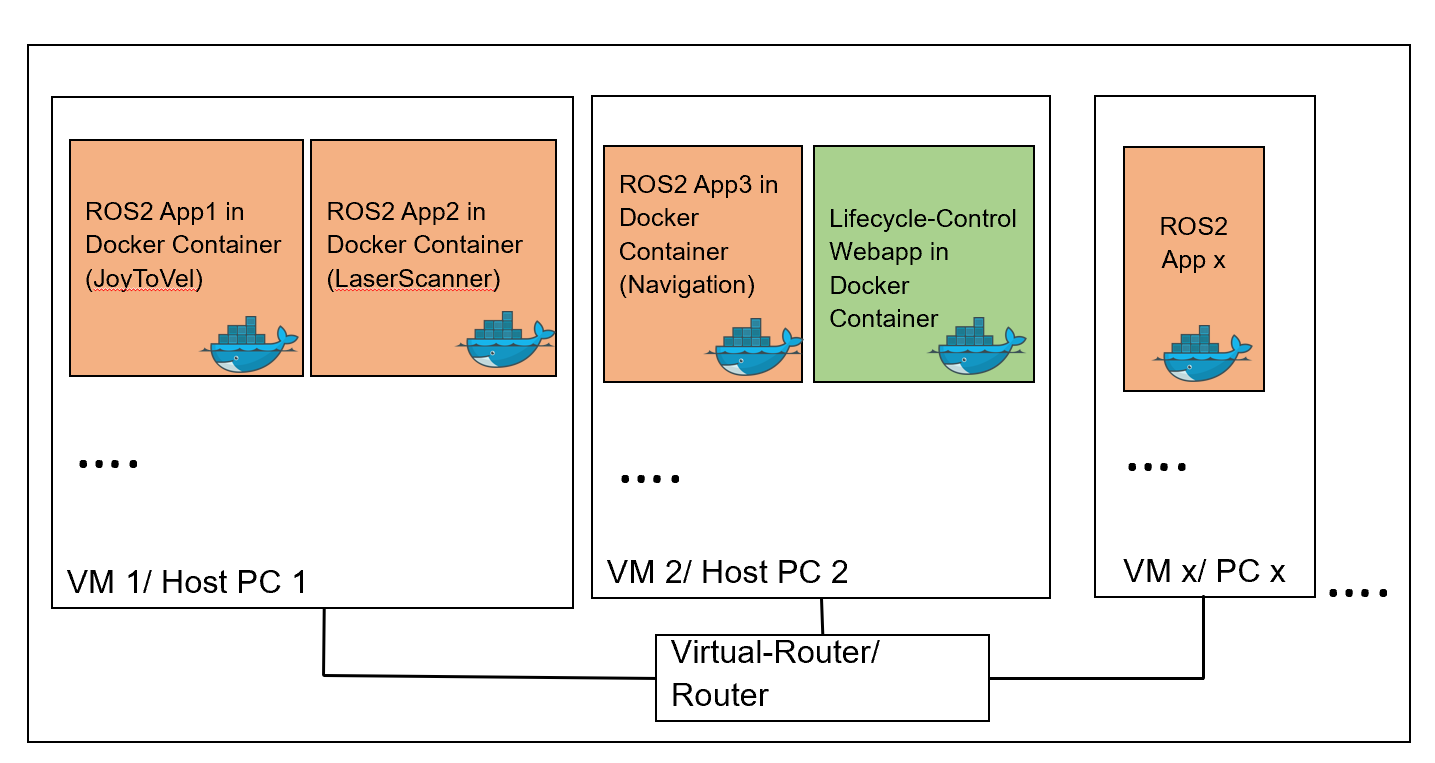
\includegraphics[width=0.95\textwidth]{"Bilder/Application-Structure.png"}
	\caption{Structure of Lifecycle Management Application}
	\label{fig:Background:LifecycleManagement}					
\end{figure}
The application consists of following major parts:

\begin{itemize}
	\item The Docker environment
	\item ROS2 Lifecycle Application
	\item Vue based Webinterface
	\item Integration
\end{itemize}

They will be explained in detail in the following section.

\section{The Docker environment}
\label{Implementierung:DockerEnvironment}
In order to develop an Industrial Edge Application, its necessary to pack an application into a Docker Image. Then it can be converted to an IE App using the Industrial Edge App Publisher.

This section describes the Docker image developed for the purposes of this thesis. A Dockerfile is used to define a Docker image. It consists of all the necessary software libraries and third party applications and precise order in which they have to installed. The following section will describe the details of the Dockerfile(structre of the Docker image) step by step.
\subsection{The Dockerfile}
\paragraph{Settng up the Base-Image} This is the first line in any Dockerfile. In this line the Ubuntu Ros Image to use is specified.
\begin{lstlisting}[language=docker,
	% caption={Dockerfile}, 
	label={code:DockerTestumgebung}]
	FROM ros:foxy-ros-core-focal
\end{lstlisting}


\paragraph{Installing Bootstrap Tools} This step installs the Bootstrap Tools(apt-utils, build-essentials, nano, git, curl, tmux) and necessary python3 extensions (python3-colcon-common-extensions, python3-colcon-mixin, python3-rosdep, python3-vcstool)

\begin{lstlisting}[language=docker,
	% caption={Dockerfile}, 
	label={code:DockerTestumgebung}]
	# install bootstrap tools
	RUN apt-get update && apt-get install -y --no-install-recommends \
		apt-utils \
		build-essential \
		nano \
		git \
		curl \
		tmux \
		inetutils-ping \
		python3-colcon-common-extensions \
		python3-colcon-mixin \
		python3-rosdep \
		python3-vcstool \
		&& rm -rf /var/lib/apt/lists/*

\end{lstlisting}

\paragraph{Setting up Ros Build environment} The rosdep is initialized and updated before installing any ROS2 Package. Then colcon mixin and metadata are setup and any relataed libraries are updated. Colcon is the default and recommended build system for ROS2. Now ROS2 applications can be built using colcon in the next step.
\begin{lstlisting}[language=docker,
	% caption={Dockerfile}, 
	label={code:DockerTestumgebung}]
	# bootstrap rosdep
	RUN rosdep init && \
	rosdep update --rosdistro $ROS_DISTRO
	# setup colcon mixin and metadata
	RUN colcon mixin add default \
		https://raw.githubusercontent.com/colcon/
		colcon-mixin-repository/master/index.yaml && \
		colcon mixin update && \
		colcon metadata add default \
		https://raw.githubusercontent.com/colcon/
		colcon-metadata-repository/master/index.yaml && \
		colcon metadata update
\end{lstlisting}

\paragraph*{Installimg necessary Ros packages} Following ROS2 Packages are instllen in this step: ros-foxy-ros-base=0.9.2-1*, ros-foxy-joy, ros-foxy-diagnostic-updater,ros-foxy-lifecycle. Depending on the type of ROS2 Appliation it might be necessary to install further Packages, which should be done in this to avoid furthr complications. Finally the system is updated to fix any broken installs and install any mising libraries.
\begin{lstlisting}[language=docker,
	% caption={Dockerfile}, 
	label={code:DockerTestumgebung}]
	# install ros2 packages
	RUN apt-get update && apt-get install -y --no-install-recommends \
		ros-foxy-ros-base=0.9.2-1* \
		ros-foxy-joy \
		ros-foxy-diagnostic-updater \
		# install for lifecycle 
		ros-foxy-lifecycle \
		nginx \
		python \
	# update system
		&& apt-get upgrade -y \
		&& rm -rf /var/lib/apt/lists/* 
\end{lstlisting}


\paragraph*{Sourcing Ros2} Sourcing is a common term among UNIX users. In order to make the desired changes applicable to the current shell , it is necessary to "source" the file. Furthermore adding sources to .bashrc files preconfigures any new shell opened. In this step ROS2 setup files are sourced so that other ROS2 commands can be run from the command line. 
\begin{lstlisting}[language=docker,
	% caption={Dockerfile}, 
	label={code:DockerTestumgebung}]
	#add sources to bashrc
	RUN echo "source /opt/ros/foxy/setup.bash" >> ~/.bashrc \
		&& echo "source /root/colcon_ws/install/setup.bash" >> ~/.bashrc
\end{lstlisting}

\paragraph*{Create and build Ros Workspace} In this step first of all the build workspace is setup, then the necessary source files are copied from external working directory to the Docker internal workspace and finally built using colcon.
\begin{lstlisting}[language=docker,
	% caption={Dockerfile}, 
	label={code:DockerTestumgebung}]
	# create and build workspace
	ENV ROS2_WS /root/colcon_ws
		
	COPY ./evo_siemensrob_ctrl ${ROS2_WS}/src/evo_siemensrob_ctrl/.
	COPY ./joy_converter ${ROS2_WS}/src/joy_converter/.
	COPY ./joytovel ${ROS2_WS}/src/joytovel/.
	COPY ./twist_mux ${ROS2_WS}/src/twist_mux/.

	RUN cd ${ROS2_WS} \
		&& . /opt/ros/foxy/setup.sh \
		&& colcon build
		
	# install RIB support
	COPY ./RIBInstall .

	RUN ./RIBInstall \
		&& rm -rf RIBInstall
\end{lstlisting}

\paragraph{Setup Node enviroment for Vue} This step installs a version of NodeJS in this Docker environment. NodeJS will be necessary to build the Vue-application and run ros2-web-bridge in forthcoming steps. 
\begin{lstlisting}[language=docker,
	% caption={Dockerfile}, 
	label={code:DockerTestumgebung}]
	# For Lifecycle-Dashboard Vue App
	ENV NODE_VERSION=12.6.0
	# Already installed RUN apt install -y curl
	RUN curl -o- https://raw.githubusercontent.com/
	creationix/nvm/v0.34.0/install.sh | bash
	ENV NVM_DIR=/root/.nvm
	RUN . "$NVM_DIR/nvm.sh" && nvm install ${NODE_VERSION}
	RUN . "$NVM_DIR/nvm.sh" && nvm use v${NODE_VERSION}
	RUN . "$NVM_DIR/nvm.sh" && nvm alias default v${NODE_VERSION}
	ENV PATH="/root/.nvm/versions/node/v${NODE_VERSION}/bin/
	:${PATH}"
	RUN node --version
	RUN npm --version
\end{lstlisting}



\paragraph{Copy package.json files to install Node Project dependencies} A package.json file is a standard package specification file for NodeJS applications. It contains all the necessary configurations and list of packages to successfully build a NodeJS aplication. In this step 
a working directory for the Vue Application is created, the the package.json is copied to the Docker internal workdirectory and finally the project depencencies are downloaded and installed.
\begin{lstlisting}[language=docker,
	% caption={Dockerfile}, 
	label={code:DockerTestumgebung}]
	# build stage
	WORKDIR /app
	COPY ./lifecycle-dashboard/package*.json ./
	RUN npm install
\end{lstlisting}

\paragraph*{Build the web app for production} The project source files for the "Lifecycle management application" are copied from external workspace to the Docker workdirectory and built for production.
\begin{lstlisting}[language=docker,
	% caption={Dockerfile}, 
	label={code:DockerTestumgebung}]
	# build stage
	COPY ./lifecycle-dashboard/ .
	RUN npm run build
\end{lstlisting}

\paragraph{Setting up a Nginx web server} In this step the nginx configuration file (described in section \ref{Impl:NginxConfig}) is copied from external workspace to the docker enviroment. The built application consisting of only .html, .css and .js files are copid to a location where nginx can easily find them and use them to start the web-application. Furthermore PORT 80 is exposed and the web-application can thus be accessed on locahost:8080 within the same network where this Docker container is running.
\begin{lstlisting}[language=docker,
	% caption={Dockerfile}, 
	label={code:DockerTestumgebung}]
	# For nginx
	COPY ./nginx.conf /etc/nginx/nginx.conf
	RUN cp -a /app/dist/. /var/www/html
	EXPOSE 80
\end{lstlisting}

\paragraph*{Installing ros2-web-bridge} In this step ros2-web-bridge is installed and other services that need to launch at startup are setup. The web-server(nginx) is setup to start at launch.
\begin{lstlisting}[language=docker,
	% caption={Dockerfile}, 
	label={code:DockerTestumgebung}]
	
	# install ros2-web-bridge

	# set workdirectory as /root
	WORKDIR /root

	#for automatic launch when container gets started 
	COPY ./dockerfile_startup.sh dockerfile_startup.sh
	RUN ["chmod", "+x", "./dockerfile_startup.sh"]
	CMD ./dockerfile_startup.sh	
\end{lstlisting}

\paragraph{Starting Ros Application} This step launches the installed ROS2-Application using its launchfile.
\begin{lstlisting}[language=bash,
	% caption={dockerfile_startup}, 
	label={code:DockerTestumgebung}]
	#!/bin/bash

	nginx
	. /opt/ros/foxy/setup.sh
	. /root/colcon_ws/install/setup.sh
	npm install ros2-web-bridge
	node node_modules/ros2-web-bridge/bin/rosbridge.js &
	ros2 launch evo_siemensrob_ctrl agv_control_launch.py 
\end{lstlisting}

\paragraph{Startup and Build scripts} Hh

% \begin{lstlisting}[language=html,
% 	caption={build_lifecycle.sh}, 
% 	label={code:DockerTestumgebung}]
% 	#!/bin/bash
% 	docker build . -t ubuntu_foxy:manual_control_rti
% 	docker run -it --privileged --network host --group-add dialout --ipc="host" --name agv_control_joy_rti ubuntu_foxy:manual_control_rti
% \end{lstlisting}

\begin{lstlisting}[language=html,
	% caption={run_lifecycle.sh}, 
	label={code:DockerTestumgebung}]
	#!/bin/bash
	docker start agv_control_joy_rti

	docker exec -it agv_control_joy_rti bash 
\end{lstlisting}

\subsection{Running multiple services in a container}
The most important running process of a container is the ENTRYPOINT and/or CMD at the end of the Dockerfile. It is generally recommended to separate areas of concern by using one service per container. This service can split into several processes (e.g. the Apache webserver starts several working processes). It is fine to have multiple processes but to get the most benefit from Docker, you should avoid having one container responsible for multiple aspects of your entire application. You can connect multiple containers via custom networks and shared volumes.

The main container process is responsible for managing all the processes it launches. In some cases, the main process is not well thought out and cannot properly terminate child processes when the container is terminated (reaping). If your process falls into this category, you can use the --init option when starting the container. The --init option adds a tiny init process as the main process in the container and takes care of reaping all processes when the container is terminated. Handling such processes is better than using a full-fledged init process like sysvinit, upstart, or systemd to manage the process lifecycle inside your container.

\begin{lstlisting}[language=bash,
	% caption={dockerfile_startup}, 
	label={code:Vue}]
	#!/bin/bash
  
	# turn on bash's job control
	set -m
	
	# Start the primary process and put it in the background
	./my_main_process &
	
	# Start the helper process
	./my_helper_process
	
	# the my_helper_process might need to know how to wait on the
	# primary process to start before it does its work and returns
	
	
	# now we bring the primary process back into the foreground
	# and leave it there
	fg %
\end{lstlisting}

\begin{lstlisting}[language=dockerfile,
	% caption={dockerfile_startup}, 
	label={code:Vue}]
	# syntax=docker/dockerfile:1
	FROM ubuntu:latest
	COPY my_first_process my_first_process
	COPY my_second_process my_second_process
	COPY my_wrapper_script.sh my_wrapper_script.sh
	CMD ./my_wrapper_script.sh
	
	
\end{lstlisting}

\lstinline{https://docs.docker.com/config/containers/multi-service_container/}


\subsection{Nginx server configuration}
\label{Impl:NginxConfig}
Configuring NGINX as a web server is about defining which URLs it processes and how it processes HTTP requests for resources at those URLs. On a deeper level, the configuration defines a set of virtual servers that control the processing of requests for specific domains or IP addresses.

Since the application in this thesis is only supposed to run within a local network (not the internet) the webserver configuration is drastically simplified. The basic HTTP settings can be left to the default configuration. Only the virtual server settings need to be configured. This section describes the configuration used for NGINX to serve static content. This includes the definition of paths searched to find requested files and set up for index files. The following listing shows the most important configurations needed to serve the developed web application on a local network.

\begin{lstlisting}[caption={Nginx configuration file (nginx.conf)}, 
	label={code:NginxConf}]
http {
	# Basic Settings
	# ...
	server {
		# listen 80 default_server;
		# listen [::]:80 default_server;

		listen       80;
		listen  [::]:80;
		server_name  localhost;

		index index.html index.htm index.nginx-debian.html;

		location / {
			# First attempt to serve request as file, then
			# as directory, then fall back to displaying a 404.
			root   /usr/share/nginx/html;
			index  index.html index.htm;
			}
		}
	}
\end{lstlisting}

A virtual server is defined by a server directive in the http context in \lstinline{nginx.conf} file. The used directives in the above configuration file are described below:

\paragraph{listen} The server configuration block usually includes a listen directive to specify the IP address and port on which the server listens for requests. Both IPv4 and IPv6 addresses are accepted; IPv6 addresses are enclosed in square brackets. In the above configuration the server listens on IP address 127.0.0.1 (localhost) and port 80.

\paragraph{server name} If there are several servers that match the IP address and port of the request, the request’s Host header field is tested against the \lstinline{server_name} directives in the server blocks. The parameter to \lstinline{server_name} can be a full name, a wildcard, or a regular expression. Since the above configuration has just one virtual server the this parameter is set to localhost.

\paragraph{root} The root directive specifies the root directory to be used to search for a file. To obtain the path of a requested file, NGINX appends the request URI to the path specified by the root directive. The directive can be placed at any level within the http {}, server {} or location {} contexts. In case the root directive is defined for a virtual server. It applies to all location {} blocks that do not contain the root directive to explicitly redefine the root.\cite{nginxCong}

\paragraph{index} If a request ends with a slash, NGINX treats it as a request for a directory and tries to find an index file in that directory. The index directive defines the name of the index file (the default is index.html). If the URI of the request is \lstinline{/some/path/}, based on the above configuration NGINX will return the file \lstinline{/usr/share/nginx/html/some/path/index.html} if it exists. If it does not, NGINX returns the HTTP code 404 (Not Found) by default. Multiple file names can be listed in the index directive. In this case, NGINX searches for the files in the specified order and returns the first file found.


\section{ROS2 Lifecycle Application}
\label{Implementierung:ROS2LifecycleApplication} 
In oder to showcase the capabilities and possible use-cases of the managed lifecycle nodes in ROS2 ecosystem a demonstration application was developed. This appliaction has multiple states which allows for reconfiguration and respawning of the node while it is running. It also is a key part for demonstrating the capabilities of the remote lifecycle management interface described in section \ref{Implementierung:VueBasedWebinterface}. This section describes the details of an example ROS2-Application with managed states and steps necessary to convert a normal ROS2-node into a managed lifecycle node. 

\subsection{Structure of a normal ROS2 publisher node}
To demonstrate the process of developing a managed lifecycle node a JoyToVel publisher node is converted into a lifecycle node in this section. The JoyToVel publisher takes input from a PlayStation4 Controller and publishes velocity and direction commands to \lstinline{\cmd_vel} topic in a ROS2 Network. Any application(node) subscribed to this topic can be controlled using this JoyToVel node.

A normal JoyToVel publisher consists of a constructor, application-specific callback functions and methods, and the main function. The necessary subscribers and publishers are initialized in the constructor. It also includes the application logic. In the main function, the node is started with the specified parameters. No changes to any parameters can be made once the node has been started. If the node crashes for some reason it has to be respawned manually. Since the JoyToVel node is an interface node, it would be beneficial to be able to dynamically reconfigure its different parameters and it demands higher reliability and stability. \\
A normal ROS2 C++ publisher node has the following structure:   
\begin{lstlisting}[language=cpp]
	#include "JoyToVel.hpp"
	namespace evo {
		//Constructor
		JoyToVel::JoyToVel() : Node("joy_to_vel")
		{
			// init subscribers
			...
			// init publishers
			...
		}

		//Callbacks and Methods
		void JoyToVel::topic_callback(const sensor_msgs::msg::Joy::SharedPtr msg) const
		{
			...
		}

		void JoyToVel::timer_callback()
		{  
			...
		}

		void JoyToVel::publishVel(const sensor_msgs::msg::Joy::SharedPtr msg)
		{
			...
		}
	}

	int main(int argc, char** argv)
	{
		rclcpp::init(argc, argv);
  
		rclcpp::spin(std::make_shared<evo::JoyToVel>());
		rclcpp::shutdown();

		return 0;
	}

\end{lstlisting}

\subsection{Structure of a ROS2 publisher node with managed lifecycle}
A lifecycle based ros2 publisher has following structure:
\begin{lstlisting}[language=cpp]
namespace evo {
  class LifecycleTalker : public rclcpp_lifecycle::LifecycleNode
  {
  public:
    /// LifecycleTalker constructor
    explicit LifecycleTalker(const std::string &node_name, bool intra_process_comms = false)
        : rclcpp_lifecycle::LifecycleNode(node_name,
                                          rclcpp::NodeOptions().use_intra_process_comms(intra_process_comms))
    {
      // init subscribers
      ....
      // init publishers
      ....
    }
  
    /// Transition callback for state configuring
    rclcpp_lifecycle::node_interfaces::LifecycleNodeInterface::CallbackReturn
    on_configure(const rclcpp_lifecycle::State &)
    {
      // Initialize and configure publishers and timers.
      pub_ = this->create_publisher<std_msgs::msg::String>("lifecycle_chatter", 10);
	  timer_ = this->create_wall_timer(
          1s, std::bind(&evo::LifecycleTalker::timer_callback, this));

      return rclcpp_lifecycle::node_interfaces::LifecycleNodeInterface::CallbackReturn::SUCCESS;
    }

    /// Transition callback for state activating
    rclcpp_lifecycle::node_interfaces::LifecycleNodeInterface::CallbackReturn
    on_activate(const rclcpp_lifecycle::State &)
    {
      // Activate the lifecycle publisher.
      pub_->on_activate();

      // Important tasks in the activating phase.
	  ....
 
      return rclcpp_lifecycle::node_interfaces::LifecycleNodeInterface::CallbackReturn::SUCCESS;
    }

    /// Transition callback for state deactivating
    rclcpp_lifecycle::node_interfaces::LifecycleNodeInterface::CallbackReturn
    on_deactivate(const rclcpp_lifecycle::State &)
    {
      // Deactivate the lifecycle publisher.
      pub_->on_deactivate();

      return rclcpp_lifecycle::node_interfaces::LifecycleNodeInterface::CallbackReturn::SUCCESS;
    }

    /// Transition callback for state cleaningup
    rclcpp_lifecycle::node_interfaces::LifecycleNodeInterface::CallbackReturn
    on_cleanup(const rclcpp_lifecycle::State &)
    {
      // Release the shared pointers to the timer and publisher. 
      timer_.reset();
      pub_.reset();

      return rclcpp_lifecycle::node_interfaces::LifecycleNodeInterface::CallbackReturn::SUCCESS;
    }

    /// Transition callback for state shutting down
    rclcpp_lifecycle::node_interfaces::LifecycleNodeInterface::CallbackReturn
    on_shutdown(const rclcpp_lifecycle::State &state)
    {
      // Tasks to be performed in shutdown phase
      ....

      return rclcpp_lifecycle::node_interfaces::LifecycleNodeInterface::CallbackReturn::SUCCESS;
    }

	// Publish method for the publisher
	void publish()
    { 
      ...
    }

    
  private:
    // This is an instance of a lifecycle publisher. This lifecycle publisher
    // can be activated or deactivated based on state of the lifecycle node
    std::shared_ptr<rclcpp_lifecycle::LifecyclePublisher<std_msgs::msg::String>> pub_;

  };

  // Application specific Callbacks/Methods
    void evo::LifecycleTalker::topic_callback(const sensor_msgs::msg::Joy::SharedPtr msg) const
    {
      	....
    }

    void evo::LifecycleTalker::timer_callback()
    {
		....
    }

    void evo::LifecycleTalker::joyCallback(const sensor_msgs::msg::Joy::SharedPtr msg)
    {
		....
    }

    void evo::LifecycleTalker::publishVel(const sensor_msgs::msg::Joy::SharedPtr msg)
    {
		....
    }
}

int main(int argc, char** argv)
{
  setvbuf(stdout, NULL, _IONBF, BUFSIZ);
  rclcpp::init(argc, argv);

  rclcpp::executors::SingleThreadedExecutor exe;
  std::shared_ptr<evo::LifecycleTalker> lc_node = std::make_shared<evo::LifecycleTalker>("lifecycle_joytovel");

  exe.add_node(lc_node->get_node_base_interface());
  exe.spin();
  rclcpp::shutdown();

  return 0;
}
\end{lstlisting}


\subsection{Conversion of a node into a Lifecycle Node}
In order to convert a normal ROS2 node into a lifecycle node following steps need to be taken:

\begin{itemize}
	\item Import necessary libraries. Following libraries are necessary for a lifecycle node. In order to import these libraries the package \lstinline{rclcpp_lifecycle and lifecycle_msgs} must be installed on the system. \begin{lstlisting}[language=cpp]
		#include <chrono>
		#include <thread>
		#include <utility>
		#include <numeric>

		#include "lifecycle_msgs/msg/transition.hpp"
		#include "rclcpp/rclcpp.hpp"
		#include "rclcpp/publisher.hpp"
		#include "rclcpp_lifecycle/lifecycle_node.hpp"
		#include "rclcpp_lifecycle/lifecycle_publisher.hpp"

		#include "rcutils/logging_macros.h"

	\end{lstlisting}
	\item Encapsulate the node in a class that inherits from class \lstinline{rclcpp_lifecycle::LifecycleNode} This brings in a series of callbacks that are called depending on the current state of the node. Each lifecycle node has a set of services associated with it that make it controllable from the outside.
	\item Initialize the public and private methods.
	\item Configure and implement transition callbacks listed in listing \ref{code:TransitionCallbacks}.
	\item Define appliation specific methods
	\item Perform necessary setup and initialization in main() function.  
\end{itemize}


\subsection{A multi node Applicaton}
A realistic robot consists of several independent components which need to run simultaneously and interact with each other. In order to simulate a system with multiple managed nodes an example multi node ROS2 Application is developed in this section. For demonstration purposes three nodes which depend on each other during different states of their lifecycle is developed. 

\section{Vue based Webinterface}
\label{Implementierung:VueBasedWebinterface}
The developed web interface is supposed to be a web version of the lifecycle management CLI. 

\subsection{Web Application Requirements}

\subsection{Web Application Design}
	\begin{figure}[H]
		\centering
		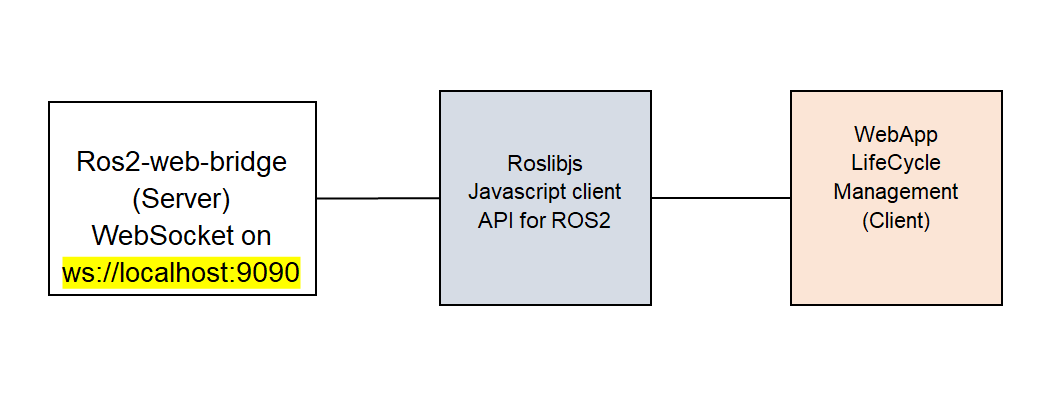
\includegraphics[width=0.95\textwidth]{"Bilder/webapp-design.png"}
		\caption{Overview of Lifecycle Management WebApp}
		\label{fig:Background:WebappDesign}					
	\end{figure}

\subsection{ROS2 Message Types/ Javascript Objects}
This section describes the ROS2 Messages and Services used to communicate with the ROS2 backend application. There was also a need to explore and examine various JavaScript counterparts to these message and service types. Messages and services  used in the developed application are listed below with their definitions. 

\paragraph{Messages:} 
\begin{itemize}
	\item \lstinline{lifecycle_msgs/msg/State}
\begin{lstlisting}[language=msg,
	caption={Message definition State}]
	# State definitions
	uint8 PRIMARY_STATE_UNKNOWN = 0
	uint8 PRIMARY_STATE_UNCONFIGURED = 1
	uint8 PRIMARY_STATE_INACTIVE = 2
	uint8 PRIMARY_STATE_ACTIVE = 3
	uint8 PRIMARY_STATE_FINALIZED = 4

	uint8 TRANSITION_STATE_CONFIGURING = 10
	uint8 TRANSITION_STATE_CLEANINGUP = 11
	uint8 TRANSITION_STATE_SHUTTINGDOWN = 12
	uint8 TRANSITION_STATE_ACTIVATING = 13
	uint8 TRANSITION_STATE_DEACTIVATING = 14
	uint8 TRANSITION_STATE_ERRORPROCESSING = 15

	## Fields

	# The state id value from the above definitions.
	uint8 id
	# A text label of the state.
	string label
\end{lstlisting}

\item \lstinline{lifecycle_msgs/msg/Transition}
\begin{lstlisting}[language=msg,
	caption={Message definition Transition}]
	# Transition id definitions
	uint8 TRANSITION_CREATE = 0
	uint8 TRANSITION_CONFIGURE = 1
	uint8 TRANSITION_CLEANUP = 2
	uint8 TRANSITION_ACTIVATE = 3
	uint8 TRANSITION_DEACTIVATE = 4
	uint8 TRANSITION_UNCONFIGURED_SHUTDOWN  = 5
	uint8 TRANSITION_INACTIVE_SHUTDOWN = 6
	uint8 TRANSITION_ACTIVE_SHUTDOWN = 7
	uint8 TRANSITION_DESTROY = 8
	uint8 TRANSITION_ON_CONFIGURE_SUCCESS = 10
	uint8 TRANSITION_ON_CONFIGURE_FAILURE = 11
	uint8 TRANSITION_ON_CONFIGURE_ERROR = 12
	uint8 TRANSITION_ON_CLEANUP_SUCCESS = 20
	uint8 TRANSITION_ON_CLEANUP_FAILURE = 21
	uint8 TRANSITION_ON_CLEANUP_ERROR = 22
	uint8 TRANSITION_ON_ACTIVATE_SUCCESS = 30
	uint8 TRANSITION_ON_ACTIVATE_FAILURE = 31
	uint8 TRANSITION_ON_ACTIVATE_ERROR = 32
	uint8 TRANSITION_ON_DEACTIVATE_SUCCESS = 40
	uint8 TRANSITION_ON_DEACTIVATE_FAILURE = 41
	uint8 TRANSITION_ON_DEACTIVATE_ERROR = 42
	uint8 TRANSITION_ON_SHUTDOWN_SUCCESS = 50
	uint8 TRANSITION_ON_SHUTDOWN_FAILURE = 51
	uint8 TRANSITION_ON_SHUTDOWN_ERROR = 52
	uint8 TRANSITION_ON_ERROR_SUCCESS = 60
	uint8 TRANSITION_ON_ERROR_FAILURE = 61
	uint8 TRANSITION_ON_ERROR_ERROR = 62
	uint8 TRANSITION_CALLBACK_SUCCESS = 97
	uint8 TRANSITION_CALLBACK_FAILURE = 98
	uint8 TRANSITION_CALLBACK_ERROR = 99
	
	## Fields

	# The transition id from above definitions.
	uint8 id
	# A text label of the transition.
	string label
\end{lstlisting}

\item \lstinline{lifecycle_msgs/msg/TransitionDescription}
\begin{lstlisting}[language=msg,
	caption={Message definition TransitionDescription}]
	# The transition id and label of this description.
	Transition transition
	# The current state from which this transition transitions.
	State start_state
	# The desired target state of this transition.
	State goal_state
\end{lstlisting}

\item \lstinline{lifecycle_msgs/msg/TransitionEvent}
\begin{lstlisting}[language=msg,
	caption={Message definition TransitionEvent}]
	# The time point at which this event occurred.
	uint64 timestamp
	# The id and label of this transition event.
	Transition transition
	# The starting state from which this event transitioned.
	State start_state
	# The end state of this transition event.
	State goal_state
\end{lstlisting}

\item \lstinline{rcl_interfaces/msg/Log}
\begin{lstlisting}[language=msg,
	label={code:ROS:Message definition Log},
	caption={Message definition Log}]
	##
	## Severity level constants
	## 
	## Since there are several other logging enumeration standard for different implementations,
	## other logging implementations may need to provide level mappings to match their internal implementations.
	##
	# Debug is for pedantic information, which is useful when debugging issues.
	byte DEBUG=10
	# Info is the standard informational level and is used to report expected
	# information.
	byte INFO=20
	# Warning is for information that may potentially cause issues or possibly unexpected
	# behavior.
	byte WARN=30
	# Error is for information that this node cannot resolve.
	byte ERROR=40
	# Information about a impending node shutdown.
	byte FATAL=50
	## Fields

	# Timestamp when this message was generated by the node.
	builtin_interfaces/Time stamp
	# Corresponding log level, see above definitions.
	uint8 level
	# The name representing the logger this message came from.
	string name
	# The full log message.
	string msg
	# The file the message came from.
	string file
	# The function the message came from.
	string function
	# The line in the file the message came from.
	uint32 line
\end{lstlisting}

\end{itemize}

\paragraph{Services:}

\begin{itemize}
	\item \lstinline{lifecycle_msgs/srv/ChangeState}
A ROS2 Service has the following structure:
\begin{lstlisting}[language=service,
	caption={Service definition ChangeState},
	label={code:ROS:Service definition ChangeState}]
	# The requested transition.
	Transition transition
	---
	# Indicates whether the state transition was successful
	bool success
\end{lstlisting}



\item \lstinline{lifecycle_msgs/srv/GetAvailableStates}
\begin{lstlisting}[language=service,
	caption={Service definition GetAvailableStates},
	label={code:ROS:Service definition GetAvailableStates}]
	---
	# Array of possible states that can be transitioned to.
	State[] available_states
\end{lstlisting}

\item \lstinline{lifecycle_msgs/srv/GetAvailableTransitions}
\begin{lstlisting}[language=service,
	caption={Service definition GetAvailableTransitions},
	label={code:ROS:Service definition GetAvailableTransitions}]
	---
	# An array of the possible start_state-goal_state transitions
	TransitionDescription[] available_transitions

\end{lstlisting}

\item \lstinline{lifecycle_msgs/srv/GetState}
\begin{lstlisting}[language=service,
	caption={Service definition GetState},
	label={code:ROS:Service definition GetState}]
	---
	# The current state-machine state of the node.
	State current_state
\end{lstlisting}

\end{itemize}



ROSLIB.ServiceRequest
ROSLIB.Service
ROSLIB.Topic


\paragraph{JavaScript Objects}
\begin{itemize}

\item ROSLIB.Service
\begin{lstlisting}[language=JavaScript,
	label={JavsScript:ROSLIB.Service}
	caption={JavaScript object definition for Service}]
	{
		ros : this.ros,
		name : `/lifecycle_node/get_state`,
		serviceType : 'lifecycle_msgs/GetState'
	}
\end{lstlisting}

\item ROSLIB.ServiceRequest
\begin{lstlisting}[language=JavaScript,
	caption={JavaScript object definition for ServiceRequest}]
	{
		requestParam1 : {requestObject1},
		requestParam2 : {requestObject2},
		...
    }
	}
\end{lstlisting}


\item ROSLIB.Topic
\begin{lstlisting}[language=JavaScript,
	caption={JavaScript object definition for Topic}]
	{
		ros : this.ros,
		name : '/rosout',
		messageType : 'rcl_interfaces/msg/Log'
	}
\end{lstlisting}
\end{itemize}

\paragraph{JSON Objects} A Javascript application uses JSON Objects to communicate over a network. A JSON object is returned when a ROS service is called or a topic is subscribed to. It is necessary to parse and process these objects to display or update information on a web page. To parse a JSON object, prior knowledge of its structure is required. \\

 \textit{JSON (JavaScript Object Notation) is a lightweight format for data exchange. Working with it is easy for humans likewise machines. It is based on a subset of the JavaScript Programming Language Standard ECMA-262 3rd Edition - December 1999. JSON is a text format that does not depend on any specific language but uses conventions familiar to the C language family, including} \lstinline{C, C++, C#, Java, JavaScript, Perl, Python}, \textit{and many others. These properties make JSON an ideal language for data exchange.}\cite{jsonDef} \\

 In the following section JSON objects used by the developed application is described in detail.
\begin{itemize}
\item  \lstinline{current_state}
\begin{lstlisting}[language=json,
	label={code:ROS:JSON state},
	caption={JavaScript object definition for \lstinline{state}}]
	{
		"current_state": {
			"id": 1,
			"label": "unconfigured"
		}
	}
\end{lstlisting}

\item \lstinline{transition}
\begin{lstlisting}[language=json,
	label={code:ROS:JSON transitoin},
	caption={JavaScript object definition \lstinline{transition}}]
	{
		"transition": {
			"id": 1,
			"label": "configure"
		},
		"start_state": {
			"id": 1,
			"label": "unconfigured"
		},
		"goal_state": {
			"id": 10,
			"label": "configuring"
		}
	}
\end{lstlisting}

\item \lstinline{available_transitions}
\begin{lstlisting}[language=json,
	label={code:ROS:JSON available transitions},
	caption={JavaScript object definition for \lstinline{available_transitions}}]
	{
		"available_transitions": [
		  {
			"transition": {
			  "id": 1,
			  "label": "configure"
			},
			"start_state": {
			  "id": 1,
			  "label": "unconfigured"
			},
			"goal_state": {
			  "id": 10,
			  "label": "configuring"
			}
		  },
		  {
			"transition": {
			  "id": 5,
			  "label": "shutdown"
			},
			"start_state": {
			  "id": 1,
			  "label": "unconfigured"
			},
			"goal_state": {
			  "id": 12,
			  "label": "shuttingdown"
			}
		  }
		]
	  }
\end{lstlisting}



\item \lstinline{available_states}
\begin{lstlisting}[language=json,
	label={code:ROS:JSON available states},
	caption={JavaScript object definition \lstinline{available_states}}]
	{
		"available_states": [
			{
			"id": 0,
			"label": "unknown"
			},
			{
			"id": 1,
			"label": "unconfigured"
			},
			...
		]
	}
\end{lstlisting}

\end{itemize}

\subsection{Used libraries/ package.json}

\subsection{Implementing Automatic State Transitions}

\subsection{Code Overview} For developing the web appliaction a web framework called VueJS (described in section \ref{Grundlagen:Vue}) is used. This allows the use of various pre-built html components and streamlined application structure with various plugins which in turn makes the UI development structured and easier. The UI part is encapsulatd inside the template tag and the JavaScript part in the script tag of a Vue component(described in section \ref{Vue:Component}). The project structure described in \ref{sec:StructureofVue.jsProject} is used.   

To secure a conection to the ROS2 backend through RosLibJS a ROSLIB.Ros Object needs to be initialized and assigned to a variable that can be accessed by all other functions in the application. This object consists of a url parameter, which will be used to assign the URL of the websocket. The websocket is made availabe by the library ros2-web-bridge. This is our main instance of RosLibJS and the same instance will be used throughout the application for working with a single Lifecycle Node. In case there are multiple Lifecycle nodes added, multiple instances of RosLibJS are created and stored. The details of the JavaScript part of the application is described below:

\paragraph{Library imports} The libraries are imported using the standard ES6 syntax. The libraries including vue-plugins to be installed are listed in the package.json file. This import syntax allows the import of the entire library or only specific components of the library. The following libraries are used:

\begin{lstlisting}[language=JavaScript,
	% caption={dockerfile_startup}, 
	label={code:Vue}]
	import * as ROSLIB from 'roslib';
	import { MDBBtn, MDBBtnGroup, MDBInput, MDBContainer, MDBRow, MDBCol } from "mdb-vue-ui-kit";
\end{lstlisting}

\paragraph{Vue Component initialization} To be able to use the imported components in the HTML-Layout they need to be initialized. The components to be used must be included within the component deirctive. Also the name of the component is assigned, this name will be used to import this component into any other component. 
\begin{lstlisting}[language=JavaScript,
	% caption={dockerfile_startup}, 
	label={code:Vue}]
	export default {
	
		name: 'LifecycleManagement',
		components: {
			MDBBtn, MDBBtnGroup, MDBInput, MDBContainer, MDBRow, MDBCol
		},
		....
	}
\end{lstlisting}

\paragraph{Declaring global variables} The data directive represents a storage of the necessary attributes for the component. All the global variables are declared in here.The original data object can be accessed with \texttt{\textcolor{purple}{this.data}} directive anywhere inside the component.
\begin{lstlisting}[language=JavaScript,
	% caption={dockerfile_startup}, 
	label={code:Vue}]
	data: function () {
		return {
			unsub: false,
			console_out: [],
			selected_logger_level: 20,
			input_node_name:"",
			added_nodes:["lifecycle_joytovel"],
			active_node: "lifecycle_joytovel",
			selected_transition: {},
			available_states: [],
			available_transitions: [],
			current_state: {},
			ros: new ROSLIB.Ros({
				url : 'ws://localhost:9090'
			})
		}
	},
\end{lstlisting}

\paragraph{Method definitions} All the functions and methods necessary for the application are to be defined inside the methods directive. All the methods used in this application are described in the section \ref{Implementation:ImportantFunctions}.
\begin{lstlisting}[language=JavaScript,
	% caption={dockerfile_startup}, 
	label={code:Vue}]
	methods: {
		...
	},
\end{lstlisting}


\paragraph{Vue instance lifecycle hook mounted} A Vue component has several lifecycle hooks (described in section \ref{Vue:Instancelifecyclehooks}), which lets a developer customize its behaviour at any specific point in its lifecycle. In this application the mounted hook is used to establish a connection to the websocket created by the ROS2-Web-Bridge.
\begin{lstlisting}[language=JavaScript,
	% caption={dockerfile_startup}, 
	label={code:Vue}]
	mounted: function () {
		var ros = new ROSLIB.Ros({
			url : 'ws://localhost:9090'
		});

		ros.on('connection', function() {
			console.log('Connected to websocket server.');
		});

		ros.on('error', function(error) {
			console.log('Error connecting to websocket server: ', error);
		});

		ros.on('close', function() {
			console.log('Connection to websocket server closed.');
		});

		this.update();
	},
\end{lstlisting}

\subsection{Important Functions/Methods}
\label{Implementation:ImportantFunctions}
Using RosLibJS the frontend application can be conected to the backend API(websocket) provided by ROS2-web-bridge. To get the required informaton about the ros2 nodes running inside the backend application several ROS2 services need to called and some ROS2 topics need to be subscribed to. The methods used to realize these functionalities are described below in detail. These methods are all included inside the \textit{methods} directive described in previous section. As described in listing \ref{{JavsScript:ROSLIB.Service} caption} a ROSLIB.Service object needs to be created everytime a service needs to be called. It has a name parameter which has the 
following syntax: 
\begin{lstlisting}
	name: '/<name of the active node>/<name of the service>'
\end{lstlisting}
This convention is utilized in all the following methods in this section.

\paragraph{Methods to add lifecycle nodes and activate it} The \lstinline{add_node} method takes in the name of the lifecycle node provided through the UI and aappends it to an array. Multiple lifecycle nodes can be added to the application using this method. To activate a node the \lstinline{set_active_node} method is called. This selects a node from an array of nodes and sets it as the active node. It also clears all the fields in the UI and updates it based on the data received for the active node. The methods for clearing and updateding the UI are described in listing \ref{Implementation:Auxillary functions}.
\begin{lstlisting}[language=JavaScript,
	% caption={dockerfile_startup}, 
	label={code:Vue}]
	add_node(){
	  if (this.input_node_name !== "") {
		this.added_nodes.push(this.input_node_name);
		console.log(this.added_nodes);
	  } 
	},

	set_active_node(data){
		this.active_node = data;
		this.clear();
		this.update();
	},
\end{lstlisting}


\paragraph{Service to get CurrentState} This method calls a ROS service to get the current state of the active lifecycle node. A new service object is created, as parameters, the global RosLibJS instance, the complete name of the service, and the service type is passed. All the available services for a lifecycle node are listed in listing \ref{code:ROS2:AvailableServices}. According to the service definition in listing \ref{code:ROS:Service definition GetState}, a ROSLIB.ServiceRequest object is created. This ServiceRequest object is then passed as a parameter to the callService function of the Service object created in the previous step.
The callService function takes three parameters:
\begin{lstlisting}
    serviceObject.callService(request, <result_handler>, <error_handler>)
\end{lstlisting}
The first parameter is the ServiceRequest object, second and third are JavaScript Arrow Functions to extract the result of the service and error message. The third parameter is optional. The structure of the result object is described in listing \ref{code:ROS:JSON state}. The current state is extracted from the result object and the global currentState variable is updated.
\begin{lstlisting}[language=JavaScript,
	% caption={dockerfile_startup}, 
	label={code:Vue}]
	srvGetCurrentState() {
		var lifecycleClient = new ROSLIB.Service({
			ros : this.ros,
			name : `/${this.active_node}/get_state`,
			serviceType : 'lifecycle_msgs/GetState'
		});

		var request = new ROSLIB.ServiceRequest({});

		lifecycleClient.callService(request, 
			(result) => {
				console.log(result);
				this.current_state = result.current_state;
			}
		)
		
		},
\end{lstlisting}

\paragraph{Service to get all available States} This method calls a ROS service to get the all available states of the active lifecycle node. A new service object is created, similar to the last example. According to the service definition in listing \ref{code:ROS:Service definition GetAvailableStates}, a ROSLIB.ServiceRequest object is created. The structure of the result object is described in listing \ref{code:ROS:JSON available states}. All available states are extracted from the result object, stored in a temporary array and the global availableStates array is updated.
\begin{lstlisting}[language=JavaScript,
	caption={Method to get available States}, 
	label={code:Vue}]
	srvGetAvailableStates() {
	  var lifecycleClient = new ROSLIB.Service({
		ros : this.ros,
		name : `/${this.active_node}/get_available_states`,
		serviceType : 'lifecycle_msgs/GetAvailableStates'
	  });

		var request = new ROSLIB.ServiceRequest({});
		var tempArr = [];

		lifecycleClient.callService(request, 
		  (result) => {
			console.log(result);
			result.available_states.forEach(element => {
				console.log(element);
				tempArr.push(element);
			});
			this.available_states = tempArr;
		})
	},

\end{lstlisting}

\paragraph{Service to get AvailableTransitions} This method calls a ROS service to get all available transitions of the active lifecycle node. A new service object is created, similar to the last example. According to the service definition in listing \ref{code:ROS:Service definition GetAvailableTransitions}, a ROSLIB.ServiceRequest object is created. The structure of the result object is described in listing \ref{code:ROS:JSON available transitions}. All available transitions are extracted from the result object, stored in a temporary array and the global availableTransitions array is updated.
\begin{lstlisting}[language=JavaScript,
	caption={Method to get available Transitions}, 
	label={code:Vue}]
	srvGetAvailableTransitions() {
	  var lifecycleClient = new ROSLIB.Service({
		ros : this.ros,
		name : `/${this.active_node}/get_available_transitions`,
		serviceType : 'lifecycle_msgs/GetAvailableTransitions'
	  });

	  var request = new ROSLIB.ServiceRequest({});
	  var tempArr = [];
	
	  lifecycleClient.callService(request, 
		(result) => {
		result.available_transitions.forEach(
			element => {
			tempArr.push(element);
		});
		this.available_transitions = tempArr;
	  })
	},
\end{lstlisting}


\paragraph{Service to ChangeState} This method calls a ROS service to change the current state of the active lifecycle node to any valid state. A new service object is created, similar to the last example. According to the service definition in listing \ref{code:ROS:Service definition ChangeState}, a ROSLIB.ServiceRequest object is created. The ServiceRequest object requires a transition parameter, which consist a transition ID and a label. Transition ID can be selected in the UI, the available selections in UI is determined by a automatic state transition logic (described in section \ref{code}). The result in this case is a boolen, which indicates if the transition was succesfull. Then the update method is called.
\begin{lstlisting}[language=JavaScript,
	% caption={dockerfile_startup}, 
	label={code:Vue}]
	srvChangeState() {
		var lifecycleClient = new ROSLIB.Service({
			ros : this.ros,
			name : `/${this.active_node}/change_state`,
			// name : '/lifecycle_joytovel/change_state', 
			serviceType : 'lifecycle_msgs/ChangeState'
		});
	
		var r_id = parseInt(this.selected_transition);

		var request = new ROSLIB.ServiceRequest({
			transition: {id: r_id, label : ""}
		});

		lifecycleClient.callService(request, function(result) {
			console.log(result);
		}, function(error) {
			console.log(error);
		});
		this.update();
	},
\end{lstlisting}

\paragraph{Subscribe to rosout} This method is necessary to implement the logging functionality in the UI. A ROSLIB.Topic object is created, which is used to subscribe to ROS topic \lstinline{\rosout}. The relevant log messages for the active lifecycle node is filtered and stored in a rolling array of a fixed size. This array is used by the logger component to disply log messages in the UI. Structure of the log message is described in listing \ref{code:ROS:Message definition Log}. The desired log level (DEBUG, INFO, WARN, ERROR or FATAL) can be selected using the mapLogLevel method in listing \ref{Implementation:Auxillary functions}. Using a global unsubscribe flag, the logging can be deactivated from the UI. 
\begin{lstlisting}[language=JavaScript,
	% caption={dockerfile_startup}, 
	label={code:Vue}]
	subscribeToRosOut(){
		var listener = new ROSLIB.Topic({
			ros : this.ros,
			name : '/rosout',
			messageType : 'rcl_interfaces/msg/Log'
			});

			var msg = [];
			listener.subscribe((msg)=> {
				this.console_out.push(msg);
				if (this.console_out.length > 10) {
					this.console_out.shift();
				}
				
				if (this.unsub) {
					listener.unsubscribe();
				}
			}) 
			console.log(msg);
		},
\end{lstlisting}

\paragraph{Auxillary Methods/Functions} These are some auxillary methods/functions used in this Vue component.
\label{Implementation:Auxillary functions}
\begin{lstlisting}[language=JavaScript,
	% caption={dockerfile_startup}, 
	label={code:Vue}]
	clear() {
		this.available_states = [];
		this.current_state = [];
		this.available_transitions = [];
	},

	update() {
		this.srvGetCurrentState()
		this.srvGetAvailableTransitions()
		this.srvGetAvailableStates()
	},

	mapLogLevel(level){
		if (level === 10) {
			return "DEBUG"
		} 
		else if (level === 20){
			return "INFO"
		}
		else if (level === 30){
			return "WARN"
		}
		else if (level === 40){
			return "ERROR"
		}
		else if (level === 10){
			return "FATAL"
		}
	}
\end{lstlisting}
% \begin{lstlisting}[language=JavaScript,
% 		% caption={dockerfile_startup}, 
% 		label={code:Vue}]
		
% 	methods: {
% 		// Available Services :
% 		// /lifecycle_joytovel/change_state
% 		// /lifecycle_joytovel/describe_parameters
% 		// /lifecycle_joytovel/get_available_states
% 		// /lifecycle_joytovel/get_available_transitions
% 		// /lifecycle_joytovel/get_parameter_types
% 		// /lifecycle_joytovel/get_parameters
% 		// /lifecycle_joytovel/get_state
% 		// /lifecycle_joytovel/get_transition_graph
% 		// /lifecycle_joytovel/list_parameters
% 		// /lifecycle_joytovel/set_parameters
% 		// /lifecycle_joytovel/set_parameters_atomically
% \end{lstlisting}

\subsection{Lifecycle Dashboard UI}

\begin{figure}[H]
	\centering
	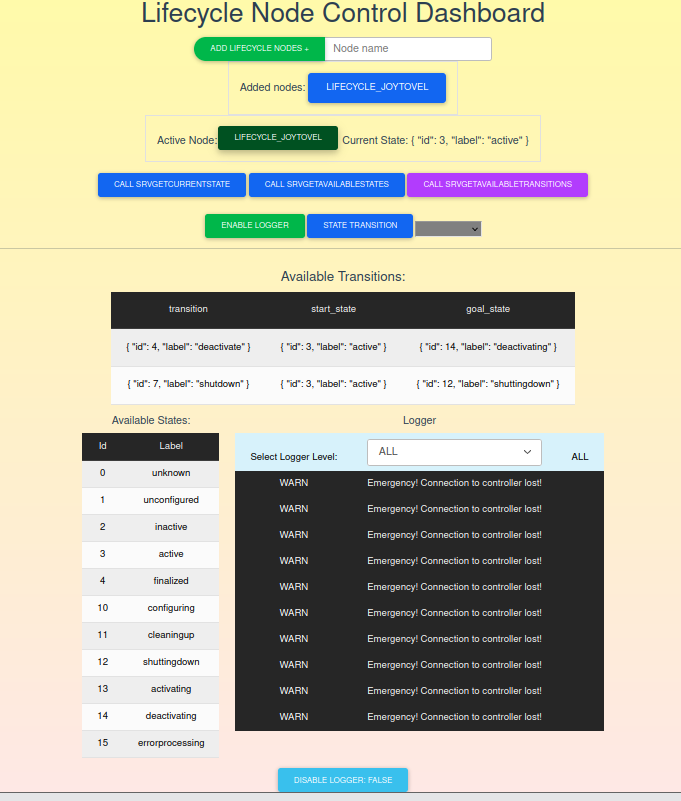
\includegraphics[width=0.95\textwidth]{"Bilder/lifecycle-dashboard.png"}
	\caption{Lifecycle Dashboard}
	\label{fig:Background:LifecycleDashboard}					
\end{figure}

\section{Integration}
\label{Implementierung:Integration}

\subsection{Conversion to Industrial Edge App} 
The Industrial Edge Publisher can be used to convert a docker image into an Industrial Edge Application. The created docker-compose.yml file (listing \ref{Implementation:dockerCompose}) is first imported into the Industrial Edge Publisher. The created images along with their various configurations are recognized by the Industrial Edge environment and these configurations are automatically applied when the app is installed on the Edge Device. No further configuration is necessary for the Edge App. Once the app has been created, it can be uploaded to the IEM using the Industrial Edge Publisher, where it is available for further distribution.

\paragraph{Docker Compose File}
With a docker-compose.yml file, services and configurations can be specified for a Docker container. This application requires several Docker containers to communicate with each other, for this purpose a seperate network is created in the docker-compose file. In addition, a volume is created to store any persistent data that might be useful for the application.

In the services section of the docker-compose file, the Docker image in the current directory is built. The name of the created Docker image is then specified. Then with the start command a \gls{ROS2} Application with lifecycle node is run. The commands \lstinline{mem_limit: 500mb} and \lstinline{restart: on-failure} are necessary for Industrial Edge. Then the docker volume created in the previous step is mounted. The network to use is specified then the docker container is connected to the network.
\begin{lstlisting}[language=docker-compose,
		caption={docker-compose.yaml used by IE Publisher},
		label={Implementation:dockerCompose}]
		networks :
 			ie-app-network :
	 			name : ie-app-network

		volumes:
			lifecycle_edge:
				name: lifecycle_edge
		
		services:
			ros2-lifecycle:
				build: ./
				image: ros2_foxy_lifecycle:1.0
				command: ros2 launch evo_siemensrob_ctrl agv_control_launch.py 
				mem_limit: 500mb
				restart: on-failure
				volumes:
					- lifecycle_edge
				networks:
					- ie-app-network		
\end{lstlisting}

		
	
\chapter{Potential Use Cases}	

To test the Lifecycle Management Interface and showcase a Use case for the Managed Lifecyle nodes a swarm of turtlesim nodes is created and various processes during their lifecycle are contorled (managed) with the help of a web based Lifecycle Management Interface. 
\subsection{Convertig Turtlesim into a Lifecycle node}

\subsection{Test Steps}
\begin{itemize}
	\item Reconfiguring the input sensitivity(in state Configure)
	\item Respawning on the Fly (transitions create, configure, activate)
	\item Shuttingdown individual Turtlesim Node (shutdown)
\end{itemize}